%%%%%%%%%%%%%%%%%%%% Client_Chapter.tex %%%%%%%%%%%%%%%%%%%%%%%%%%%%%%%%%%%
%
% This file includes the Client chapter for the AudioFiles DCCP whitepaper
%
% author: William McVicker
%
%%%%%%%%%%%%%%%% Springer %%%%%%%%%%%%%%%%%%%%%%%%%%%%%%%%%%


% RECOMMENDED %%%%%%%%%%%%%%%%%%%%%%%%%%%%%%%%%%%%%%%%%%%%%%%%%%%
%\documentclass[graybox]{svmult}
\documentclass[letterpaper, 9 pt, balance, conference]{ieeeconf} 

\usepackage{float}
\usepackage{amsmath}        % need for equations
\usepackage{mathptmx}       % selects Times Roman as basic font
\usepackage{helvet}         % selects Helvetica as sans-serif font
\usepackage{courier}        % selects Courier as typewriter font
%
\usepackage{makeidx}         % allows index generation
\usepackage{graphicx}        % standard LaTeX graphics tool
\usepackage{subfig}
                             % when including figure files
\usepackage{multicol}        % used for the two-column index
\usepackage{balance}
% see the list of further useful packages
% in the Reference Guide

\makeindex             % used for the subject index
                       % please use the style svind.ist with
                       % your makeindex program

\newcommand{\thickhline}{\noalign{\hrule height 1.0pt}}
\newcommand{\tab}{$\hspace{6pt}$}
\newcommand{\mathbi}[1]{\textbf{\em #1}}
%%%%%%%%%%%%%%%%%%%%%%%%%%%%%%%%%%%%%%%%%%%%%%%%%%%%%%%%%%%%%%%%%%%%%%%%%%%%%%%%%%%%%%%%%

\begin{document}

\bibliographystyle{IEEEtran}

\title{Audio Data Transmission using DCCP Transport Protocol}

\author{\authorblockN{Chris Hoover\authorrefmark{1}, Tim Biggs\authorrefmark{1}, William McVicker\authorrefmark{1}}$\vspace{3pt}$
\authorblockA{\authorrefmark{1}California Polytechnic State University\\
   San Luis Obispo, CA 93407 USA\\%
   Email: chhover@, tebiggs@, wmcvicke@calpoly.edu}%
}

\maketitle
\IEEEpeerreviewmaketitle

\begin{abstract}
\boldmath 
This paper aims to build a framework that utilizes the Data Congestion Control Protocol (DCCP) in order to experimentally test its congestion control system.  DCCP is a hybrid between TCP and UDP in that it offers congestion control across an unreliable transmission protocol along with a connection-oriented setup and teardown design. Applications that do not require a reliable connection, but desire to trasmit data at high rates are the ideal users of DCCP, i.e. audio streaming, video streaming, and video games. This paper proposes the design of an audio chatting application that has a framework capable of swapping out different transport layer protocols.  Specifically, three protocols were selected: DCCP, TCP, and UDP.  By abstracting out the transport layer at the application level, we can easily compare and contrast the differences in jitter and packet loss between the three different transport layer protocols in an audio streaming/chatting environment.

\end{abstract}

\section{Introduction}
\label{sec:intro}

Data Congestion Control Protocol (DCCP) is a transport layer protocol that
implements congestion control over an unreliable network~\cite{kohler06}. 
This protocol is a hybrid between UDP and TCP in that it contains the benefits
of unreliability provided by UDP along with the congestion control system found in 
TCP. DCCP originated due to the problem that occurs when transmitting data
at high rates across a network with overloading background traffic. In this
scenario, UDP will continue to transmit packets over the network, which will 
likely be dropped and increase network congestion while TCP would increasingly
slow down and continue to try and resend packets that may not be relevant by 
the time they arrive at their destination such as in meadia streaming 
applications.

The main goal of this paper is to evaluate DCCP's congestion control performance
by implementing a voice chatting application with DCCP as the underlying audio
transmission protocol.  The voice chatting framework was designed to allow the
user, upon running the application, choose between DCCP, UDP, and TCP as the
transport layer protocol of choice for transmitting audio packets. This is done
by building a framework that abstracts out the transport layer protocol at the
application layer. With this framework, we can observe differences in speed, 
jitter, and packet loss.


\section{Background}
\label{sec:backg}

The most popular transport layer protocols in use are TCP and UDP.  Both of these
protocols have their places in the networks realm and perform well under their 
respective applications.  TCP is known mainly for it reliability along with its
congestion control system while UDP favors timeliness over reliability.  With the
increase in media streaming over the past decade, the idea of timeliness has
become a very important feature.  We as humans, would rather compromise video
quality for synchronized audio and video mainly due to our abilities to deduce
information from segments of information.  Therefore, using a protocol such as UDP
that doesn't worry about loosing a few packets over time is preferred for this type 
of application.  However, when transmitting data that would be corrupt if pieces 
were lost, a reliable protocol must be used to maintain file integrity.  TCP was
designed for this very reason and is widely used as the standard reliable transport
layer protocol.

Even though both of these protocols cover the two extremes: reliable and unreliable
networks, at times a hybrid of the two is desireable.  A situation
that may arise is when media streaming occurs on a congested network. 
Congested networks cause extreme amounts of delay to TCP connections because of
the increased packet loss and the recovery TCP takes to maintain its reliability. 
So using TCP automatically is removed from the desireable options.  For
UDP connections, we can see that there is no traffic speed limit to restrict the
transmission rate UDP utilizes aside from the physical restrictions.  Therefore, 
applications that use UDP actually
may cause a network to become congested due to the high bursts that occur when
trasmitting large blocks of data.  Streaming video with encoding is a good example 
of applications that cause a varying datagram size, specifically MPEG's key frames
verus incremental frames.

DCCP was designed for this very purpose: to support congestion control on an 
unreliable network.  Not only do the authors of DCCP succesfully implement an 
unreliable transport layer protocol with congestion control support, but it also 
sheds light on the complexity of TCP.

\section{Architecture}
\label{sec:architec}

The voice chatting application was designed to work with many different clients
that communicate with a central server to retrieve information about how to call
other clients as well as the current status of the user's friends. The server 
maintains a database used to authenticate each user upon starting the application.
After logging into the system, the server is used as an intermediary for the clients
to retrieve current information about the user's friends' status, hostname, and
port number. This information can be used to request a chatting session with another
client that is logged onto the server.  Fig.~\ref{fig:setup} shows a high-level
network topology representation of what a set of clients logged into this chatting 
application would look like.  The server and client subsystems are described in
the following subsections.

\begin{figure}[h]
   \centering
      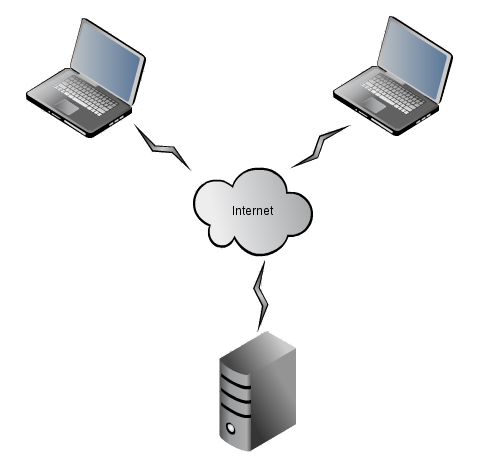
\includegraphics[width=0.4\textwidth]{pics/setup}
   \caption{High-level diagram of how the voice chatting application is setup.}
\label{fig:setup}
\end{figure}


\subsection{Server Design}
\label{subsec:server_des}

<Tim should add his stuff here>

\subsection{Client Design}
\label{subsec:client_des}

\begin{figure*}[!t]
   \centering
      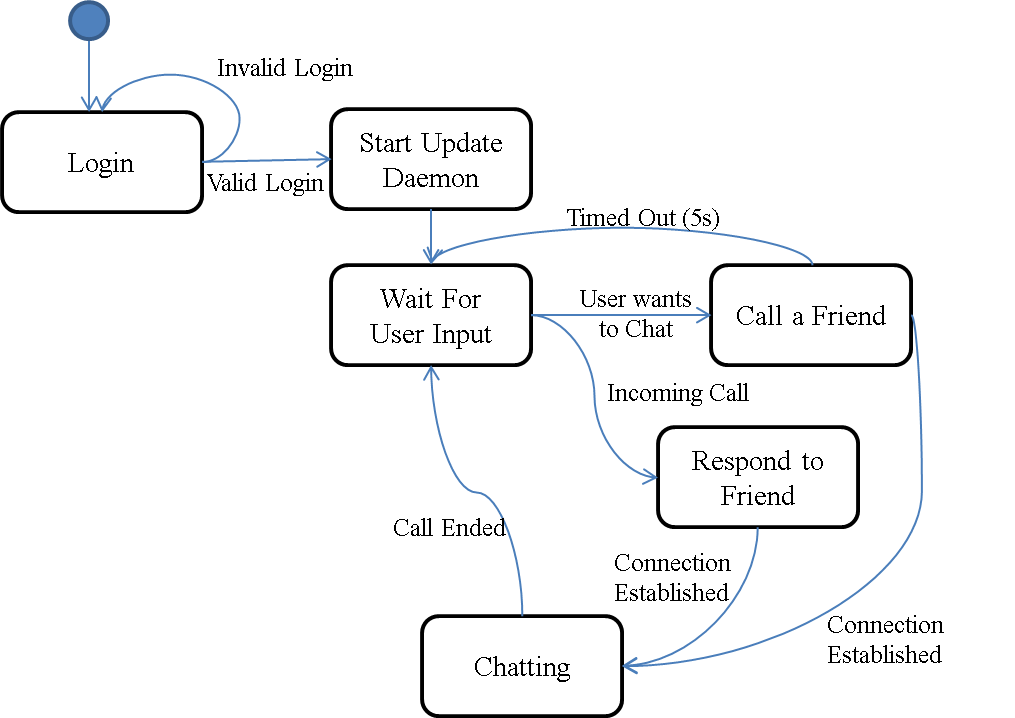
\includegraphics[width=0.8\textwidth]{pics/Client_StateDiagram}
   \caption{Client State Diagram demonstrating the general flow on the client-side.}
\label{fig:client_state_diag}
\end{figure*}

The client application is the core of the voice chatting system.  It initiates all
the communication with the server in order to receive the user's personal 
information which includes a friends list. For purposes of this paper, a friend
is one whom appears on the list of people a user can call. The application currently
does not support the ability for users to add friends during run-time.  Once the 
user logs into the server,
the client has free roam to make outgoing calls or answer incoming calls.  This
application only supports one-to-one chatting with a notification system that 
indicates when a friend is calling while the user is chatting with another client.  

The client-side of the system handles all the audio transmission between clients
as well as manages the setup and teardown of the transport protocol used to
communicate between two clients.  Each client is fitted with a transport protocol
object that handles all the layer three calls which send and receive data between
two clients using sockets.  The specific transport layer protocol is determined
upon loading the application by the user where DCCP, UDP, and TCP are the three
options. Each client is capable of calling friends as well as accepting calls from
other clients.  This requires a \textit{server} and \textit{client} model present
on each client's machine in order to monitor a socket for incoming calls as well
as open a new socket for outgoing calls.  Fig.~\ref{fig:client_state_diag} gives 
a state diagram representation of the client-side system.


The client communicates with the server once upon logging into the system and again
every time a client wants to call a friend.  When making an outgoing call,
the client asks the server for the hostname and port number of the friend he or
she wants to call.  This information is relayed back to the requestor which is then
used to directly call the friend of interest.  Since all communication with the
server contains important information about how to contact others within the 
network, the connection needs to be reliable; therefore, TCP is used for all 
communication between the clients and the server. Additionally, a seperate thread
is started immediately after logging into the server that handles receiving
periodic messages from the server which indicate any changes in the user's friends'
statuses. 


\subsection{Transport Layer Abstraction}
\label{subsec:transport_abs}

The main feature of this voice chatting application is its ability to easily 
swap in and out different transport layer protocols.  Essentially, this application
is a framework for testing the behavior of transport layer protocols with an
audio streaming application.  The abstraction was designed using the concept of
polymorphism.  Basically, a class called \textit{TransProtocol} was constructed
with several virtual functions that inhereting children must implement, i.e. DCCP,
TCP, and UDP.  These include the following:

\begin{itemize}
   \item{initMaster(uint16\_t)}
   \item{initSlave(char *, uint16\_t)}
   \item{sendPacket(void *, size\_t)}
   \item{recvPacket(void *, size\_t, int flags)}
   \item{getCallerID()}
   \item{ignoreCaller()}
   \item{answerCall()}
   \item{endCall()}
\end{itemize}

The above functions need to be implemented individually according to the specific
transport layer protocol.  For example, DCCP and TCP are connection-oriented and
need to setup a connection between two computers initially before any data packets 
can be transmitted whereas UDP connections open a socket and wait for 
whomever decides to send data its way.  The initialization steps for each of the
different transport layer protocols occur in the functions \textit{initMaster} and
\textit{initSlave}.  These two functions differ in the way the sockets are handled.

For the \textit{initMaster} function, the socket is bound to a randomly selected 
port in the same manner as the server does in a traditional server-client TCP model.
This port is then configured to listen for incoming requests. 
Before any clients can call this user, the port number needs to be reported to
the central server which saves it to a database. This port is continuously 
monitored by the client to notify the user of any incoming calls.  When an incoming
call is detected, the client machine accepts the call and extracts the caller's 
identification from the first packet to determine who the caller is using the 
\textit{getCallerID} function.  At this point, the user is notified that an 
incoming request has been received and is given the option to accept or decline
the call.  The appropriate action is taken based on the users response.

The \textit{initSlave} function is used when a client wants to make an outgoing
call to a friend.  For this to occur, the client machine requests from the central 
server the hostname and port number of the friend he or she wants to call 
identified by the user identification number.  After retrieving the proper contact 
information from the central server, \textit{initSlave} opens a socket to 
communicate with the friend.  Similar to the \textit{initMaster} function, if the
callee accepts the users call, then the chatting state will be entered and audio
capturing and playback will begin while being transferred across the transport
layer protocol of choice.

To handle processing the audio transmission and incoming chatting requests, the
main application was multi-threaded using boost threads.  Basically, the main
application thread handles the incoming requests and parses through the first
incoming request packets to identify who the caller is.  Once a connection
is established between two clients and the callee accepts the call, a chatting
thread is spawned that handles the audio capturing and playback along with the 
packet construction and transmission.  Within the chatting thread, there is an
audio playback thread started, which is discussed in the next section.



\subsection{Audio Processing}
\label{subsec:audio_proc}

Audio transmission was handled in the simplest possible manner.  The ALSA libraries
were used to capture and playback the raw audio from the microphone on each of the 
client's machines.  The ALSA libraries were used because of their simplicity and
built-in linux functionality.   

The audio was captured at 8,000 bytes per second on 2 channels.  In a 
single packet, 1,400 bytes are transmitted.  The capture and transmission of audio 
data occurs in the main chatting thread while the playback of the received audio 
packets occurr in a seperate thread.  This thread is dedicated to reading from
a buffer that contains received audio packets.  To reduce the latency 
introduced by transmitting in real-time over a network, a minimum buffer size
threshold is set.


\section{Results}
\label{sec:results}

To evaluate how well DCCP's congestion control system works, we designed an 
experiment to run using each of the three different transport layer protocols. This
goal of the experiments were to analyze jitter and packet loss.  These two
measurements should give a good estimate on the quality of the connection and
the performance gain or loss by using congestion control versus not using it.  

...more results and graphs and data :)

\section{Conclusion}
\label{sec:concl}

From the results we can see that ....

\balance
\bibliography{references}
\end{document}
